\section{Komplexität}
\label{KomplexSect}

Für viele ständig auftretende Berechnungsprobleme, wie Sortieren, die
arithmetischen Operationen (Addition, Multiplikation, Division),
Fourier-Transformation etc., sind sehr effiziente Algorithmen
konstruiert worden. Für wenige andere praktische Probleme weiß man,
dass sie nicht oder nicht effizient algorithmisch lösbar sind. Im
Gegensatz dazu ist für einen sehr großen Teil von Fragestellungen aus
den verschiedensten Anwendungsbereichen wie Operations Research,
Netzwerkdesign, Programmoptimierung, Datenbanken,
Betriebssystem-Entwicklung und vielen mehr jedoch nicht bekannt, ob
sie effiziente Algorithmen besitzen (vgl.~die Abbildungen
\ref{NPVollProbs1} und \ref{NPVollProbs2}). Diese Problematik hängt
mit der seit über vierzig Jahren\footnote{Interessanterweise reicht die Geschichte des $\P\stackrel{?}{=}\NP$-Problems viel weiter in die Geschichte zurück. So fragte 1956 Kurt Gödel in einem Brief an John von Neumann schon "`Given a first-order formula $F$ and a natural number $n$, determine if there is a proof of $F$ of length $n$"'. Gödel war an der Anzahl von Schritten interessiert, die eine Turing-Maschine benötigt, um dieses Problem zu lösen. Dazu fragte er, ob dies in linearer oder quadratischer Zeit möglich ist, was man als eine Frühform der $\P\stackrel{?}{=}\NP$-Frage auffassen könnte.} offenen $\P\stackrel{?}{=}\NP$-Frage
zusammen, wahrscheinlich gegenwärtig das wichtigste ungelöste Problem
der theoretischen Informatik. Es wurde sogar vor einiger Zeit auf Platz 1 der
Liste der so genannten \emph{Millennium Prize Problems} des Clay
Mathematics Institute gesetzt\footnote{siehe \url{http://www.claymath.org/millennium-problems}}.  
Diese Liste umfasst sieben offene Probleme aus der gesamten
Mathematik. Das Clay Institute zahlt jedem, der eines dieser Probleme 
löst, eine Million US-Dollar.

In diesem Abschnitt werden die wesentlichen Begriffe aus dem Kontext
des $\P\stackrel{?}{=}\NP$-Problems und des Begriffes der
$\NP$-Vollständigkeit erläutert, um so die Grundlagen für das
Verständnis derartiger Probleme zu schaffen und deren Beurteilung zu
ermöglichen.

\subsection{Effizient lösbare Probleme: die Klasse $\mathbf{P}$}

Jeder, der schon einmal mit der Aufgabe konfrontiert wurde, einen
Algorithmus für ein gegebenes Problem zu entwickeln, kennt die
Hauptschwierigkeit dabei: Wie kann ein effizienter Algorithmus
gefunden werden, der das Problem mit möglichst wenigen Rechenschritten
löst? Um diese Frage beantworten zu können, muss man sich zunächst
einige Gedanken über die verwendeten Begriffe, nämlich "`Problem"',
"`Algorithmus"', "`Zeitbedarf"' und "`effizient"', machen.

Was ist ein "`Problem"'? Jedem Programmierer ist diese Frage intuitiv
klar: Man bekommt geeignete Eingaben, und das Programm soll die
gewünschten Ausgaben ermitteln. Ein einfaches Beispiel ist das Problem
MULT. (Jedes Problem soll mit einem eindeutigen Namen versehen und
dieser in Großbuchstaben geschrieben werden.) Hier bekommt man zwei
ganze Zahlen als Eingabe und soll das Produkt beider Zahlen berechnen,
d.h.~das Programm berechnet einfach eine zweistellige Funktion. Es hat
sich gezeigt, dass man sich bei der Untersuchung von Effizienzfragen
auf eine abgeschwächte Form von Problemen beschränken kann, nämlich
sogenannte \dindex{Entscheidungsprobleme}. Hier ist die Aufgabe, eine
gewünschte Eigenschaft der Eingaben zu testen. Hat die aktuelle
Eingabe die gewünschte Eigenschaft, dann gibt man den Wert $1$
($\triangleq$ \texttt{true}) zurück
(man spricht dann auch von einer 
\dindex{positiven Instanz}\index{Instanz!positiv} des Problems), hat 
die Eingabe die Eigenschaft nicht, dann gibt man den Wert $0$
($\triangleq$ \texttt{false}) zurück. Oder anders formuliert: Das
Programm berechnet eine Funktion, die den Wert 0 oder 1 zurück gibt
und partitioniert damit die Menge der möglichen Eingaben in zwei
Teile: die Menge der Eingaben mit der gewünschten Eigenschaft und die
Menge der Eingaben, die die gewünschte Eigenschaft nicht
besitzen. Folgendes Beispiel soll das Konzept verdeutlichen:

\prob{PARITY}
{Positive Integerzahl $x$}
{Ist die Anzahl der Ziffern 1 in der Binärdarstellung von $x$ ungerade?}

Es soll also ein Programm entwickelt werden, das die Parität einer
Integerzahl $x$ berechnet. Eine mögliche Entscheidungsproblem-Variante
des Problems MULT ist die folgende:

\goodbreak
\prob{$\mathrm{MULT}_\mathrm{D}$}
{Integerzahlen $x,y$, positive Integerzahl $i$}
{Ist das $i$-te Bit in $x\cdot y$ gleich $1$?}
Offensichtlich sind die Probleme MULT und MULT$_\mathrm{D}$ gleich schwierig (oder
leicht) zu lösen.



\begin{wrapfigure}[14]{r}{5cm}
\centerline{\includegraphics[scale=0.7]{niko.eps}}
\caption{Der Graph $G_N$}
\label{nikolaus} 
\end{wrapfigure}
Im Weiteren wollen wir uns hauptsächlich mit Problemen beschäftigen,
die aus dem Gebiet der Graphentheorie stammen.  Das hat zwei
Gründe. Zum einen können, wie sich noch zeigen wird, viele praktisch
relevante Probleme mit Hilfe von Graphen modelliert werden, und zum
anderen sind sie anschaulich und oft relativ leicht zu verstehen.  Ein
(ungerichteter) Graph $G$ besteht aus einer Menge von Knoten $V$ und
einer Menge von Kanten $E$, die diese Knoten verbinden. Man schreibt:
$G=(V,E)$. Ein wohlbekanntes Beispiel ist der Nikolausgraph:
$G_N=\bigl(\{1,2,3,4,5\},\allowbreak\{(1,2),\allowbreak(1,3),\allowbreak
(1,5),\allowbreak(2,3),\allowbreak(2,5),\allowbreak(3,4),\allowbreak
(3,5),\allowbreak(4,5)\}\bigr)$.  Es gibt also fünf Knoten
$V=\{1,2,3,4,5\}$, die durch die Kanten in
$E=\{(1,2),\allowbreak(1,3),\allowbreak(1,5),\allowbreak(2,3),\allowbreak
(2,5),\allowbreak(3,4),\allowbreak(3,5),\allowbreak(4,5)\}$ verbunden
werden (siehe Abbildung \ref{nikolaus}).


Ein prominentes Problem in der Graphentheorie ist es, eine sogenannte
Knotenfärbung zu finden. Dabei wird jedem Knoten eine Farbe
zugeordnet, und man verbietet, dass zwei Knoten, die durch eine Kante
verbunden sind, die gleiche Farbe zugeordnet wird. Natürlich ist die
Anzahl der Farben, die verwendet werden dürfen, durch eine feste
natürliche Zahl $k$ beschränkt. Genau wird das Problem, ob ein Graph
$k$-färbbar ist, wie folgt beschrieben:

\prob{$k\mathrm{COL}$}
{Ein Graph $G=(V,E)$}
{Hat $G$ eine Knotenfärbung mit höchstens $k$ Farben?}

Offensichtlich ist der Beispielgraph $G_N$ nicht mit drei Farben färbbar
(aber mit $4$ Farben, wie man leicht ausprobieren kann), und jedes
Programm für das Problem $3\mathrm{COL}$ müsste ermitteln, dass $G_N$ die
gewünschte Eigenschaft ($3$-Färbbarkeit) nicht hat.

Man kann sich natürlich fragen, was das künstlich erscheinende
Problem $3\mathrm{COL}$ mit der Praxis zu tun hat. Das folgende einfache
Beispiel soll das verdeutlichen. Man nehme das Szenario an, dass
ein großer Telefonprovider in einer Ausschreibung drei
Funkfrequenzen für einen neuen Mobilfunkstandard erworben hat. Da er
schon über ein Mobilfunknetz verfügt, sind die Sendemasten schon
gebaut. Aus technischen Gründen dürfen Sendemasten, die zu eng stehen,
nicht mit der gleichen Frequenz funken, da sie sich sonst stören
würden. In der graphentheoretischen Welt modelliert man die
Sendestationen mit Knoten eines Graphen, und "`nahe"' zusammenstehende
Sendestationen symbolisiert man mit einer Kante zwischen den Knoten,
für die sie stehen. Die Aufgabe des Mobilfunkplaners ist es nun, eine
$3$-Färbung für den entstehenden Graphen zu finden. Offensichtlich
kann das Problem verallgemeinert werden, wenn man sich nicht auf drei
Farben/Frequenzen festlegt; dann aber ergeben sich genau die oben
definierten Probleme $k\mathrm{COL}$ für beliebige Zahlen $k$.

Als nächstes ist zu klären, was unter einem "`Algorithmus"' zu
verstehen ist. Ein Algorithmus ist eine endliche, formale Beschreibung
einer Methode, die ein Problem löst (z.B.~ein Programm in einer
beliebigen Programmiersprache). Diese Methode muss also alle Eingaben
mit der gesuchten Eigenschaft von den Eingaben, die diese Eigenschaft
nicht haben, unterscheiden können. Man legt fest, dass der Algorithmus
für erstere den Wert $1$ und für letztere den Wert $0$ ausgeben
soll. Wie soll die "`Laufzeit"' eines Algorithmus gemessen werden? Um
dies festlegen zu können, muss man sich zunächst auf ein sogenanntes
\dindex{Berechnungsmodell} festlegen. Das kann man damit vergleichen,
welche Hardware für die Implementation des Algorithmus verwendet
werden soll. Für die weiteren Analysen soll das folgende einfache
C-artige Modell verwendet werden: Es wird (grob!) die Syntax von C
verwendet und festgelegt, dass jede Anweisung in einem Schritt
abgearbeitet werden kann. Gleichzeitig beschränkt man sich auf zwei
Datentypen: einen Integer-Typ und zusätzlich Arrays dieses
Integer-Typs (wobei Array-Grenzen nicht deklariert werden müssen,
sondern sich aus dem Gebrauch ergeben). Dieses primitive
Maschinenmodell ist deshalb geeignet, weil man zeigen kann, dass jeder
so formulierte Algorithmus auf realen Computern implementiert werden
kann, ohne eine substantielle Verlangsamung zu erfahren.  
%
(Dies gilt zumindest, wenn die verwendeten Zahlen nicht
übermäßig wachsen, d.h., wenn alle verwendeten Variablen nicht zu viel
Speicher belegen. Genaueres zu dieser Problematik -- man spricht von
der Unterscheidung zwischen \dindex{uniformem Komplexitätsmaß} und
\dindex{Bitkomplexität} -- findet sich in \cite[S.~62f]{Sch01}.)

Umgekehrt kann man ebenfalls sagen, dass dieses einfache Modell die
Realität genau genug widerspiegelt, da auch reale Programme ohne allzu
großen Zeitverlust auf diesem Berechnungsmodell simuliert werden
können. Offensichtlich ist die \emph{Eingabe} der Parameter, von dem
die Rechenzeit für einen festen Algorithmus abhängt. In den
vergangenen Jahrzehnten, in denen das Gebiet der Analyse von
Algorithmen entstand, hat die Erfahrung gezeigt, dass die Länge der
Eingabe, also die Anzahl der Bits, die benötigt werden um die Eingabe
zu speichern, ein geeignetes und robustes Maß ist, in der die
Rechenzeit gemessen werden kann. Auch der Aufwand, die Eingabe selbst
festzulegen (zu konstruieren), hängt schließlich von ihrer Länge ab,
nicht davon, ob sich irgendwo in der Eingabe eine $0$ oder $1$
befindet.

\subsubsection{Das Problem der 2-Färbbarkeit}
Das Problem der 2-Färbbarkeit ist wie folgt definiert:

\prob{$2\mathrm{COL}$}
{Ein Graph $G=(V,E)$}
{Hat $G$ eine Knotenfärbung mit höchstens $2$ Farben?}
Es ist bekannt, dass dieses Problem mit einem sogenannten
\dindex{Greedy-Algorithmus} gelöst werden kann: Beginne mit einem
beliebigen Knoten in $G$ (z.B.~$v_1$) und färbe ihn mit Farbe 1. Färbe
dann die Nachbarn dieses Knoten mit 2, die Nachbarn dieser Nachbarn
wieder mit 1, usw.  Falls $G$ aus mehreren Komponenten
(d.h.~zusammenhängenden Teilgraphen) besteht, muss dieses Verfahren
für jede Komponente wiederholt werden. $G$ ist schließlich 2-färbbar,
wenn bei obiger Prozedur keine inkorrekte Färbung entsteht. Diese Idee
führt zu Algorithmus \ref{TColAlgo}.

Die Laufzeit von Algorithmus \ref{TColAlgo} kann wie folgt abgeschätzt
werden: Die erste \textbf{for}-Schleife benötigt $n$ Schritte.  In der
\textbf{while}-Schleife wird entweder mindestens ein Knoten gefärbt
und die Schleife dann erneut ausgeführt, oder es wird kein Knoten
gefärbt und die Schleife dann verlassen; also wird diese Schleife
höchstens $n$-mal ausgeführt. Innerhalb der \textbf{while}-Schleife
finden sich drei ineinander verschachtelte \textbf{for}-Schleifen, die
alle jeweils $n$-mal durchlaufen werden, und eine
\textbf{while}-Schleife, die maximal $n$-mal durchlaufen wird.

Damit ergibt sich also eine Gesamtlaufzeit der Größenordnung $n^4$,
wobei $n$ die Anzahl der Knoten des Eingabe-Graphen $G$ ist. Wie groß
ist nun die Eingabelänge, also die Anzahl der benötigten Bits zur
Speicherung von $G$?  Sicherlich muss jeder Knoten in dieser
Speicherung vertreten sein, d.h.~also, dass mindestens $n$ Bits zur
Speicherung von $G$ benötigt werden. Die Eingabelänge ist also
mindestens $n$. Daraus folgt, dass die Laufzeit des Algorithmus also
höchstens von der Größenordnung $N^4$ ist, wenn $N$ die Eingabelänge
bezeichnet.

\goodbreak
\RestyleAlgo{ruled}
\begin{algorithm}
\caption{Algorithmus zur Berechnung einer $2$-Färbung eines Graphen}
\label{TColAlgo}
%
\KwData{Graph $G = (\{v_1, \dots v_n\}, E)$;}
\KwResult{$1$ wenn es eine $2$-Färbung für $G$ gibt, $0$ sonst}
\BlankLine
\Begin{
\For{$($$i = 1$ to $n$$)$}{
$\mathrm{Farbe}[i] = 0$\;
}
\BlankLine
$\mathrm{Farbe}[1] = 1$\;
\Repeat{$(\mathrm{aktKompoBearbeiten})$}{
  aktKompoBearbeiten = \texttt{false}\;
  \For{$($$i = 1$ $\mathrm{to}$ $n$$)$}{
    \For{$($$j = 1$ $\mathrm{to}$ $n $$)$}{
      \tcc*[f]{Kante mit noch ungefärbten Knoten?}

      \If{$(($$(v_i,v_j) \in E$$)$ und $(\mathrm{Farbe}[i] \not= 0$$)$ und 
          $(\mathrm{Farbe}[j] = 0$$))$}{
        \tcc*[f]{$v_j$ bekommt eine andere Farbe als $v_i$}
      
        $\mathrm{Farbe}[j] = 3 - \mathrm{Farbe}[i]$\;
        aktKompoBearbeiten = \texttt{true}\;
        \tcc*[f]{Alle direkten Nachbarn von $v_j$ prüfen}

        \For{$($$k = 1$ $\mathrm{to}$ $n $$)$}{
          \tcc*[f]{Kollision beim Färben aufgetreten?}

          \If{$(($$(v_j,v_k) \in E$$)$ und 
              $(\mathrm{Farbe}[i] = \mathrm{Farbe}[k]$$))$}{
            \tcc*[f]{Kollision! Graph nicht $2$-färbbar}

            \Return $0$\;
          }
        } 
      }
    }
  }
  \tcc*[f]{Ist die aktuelle Zusammenhangskomponente völlig gefärbt?}

  \If{$(\mathrm{not(aktKompoBearbeiten)})$}{
    $i = 1$\;
    \tcc*[f]{Suche nach einer weiteren Zusammenhangskomponente von $G$}

    \Repeat{$(\mathrm{not(weiterSuchen)}$ $\mathrm{und}$ $(i \le n))$}{
      \tcc*[f]{Liegt $v_i$ in einer neuen Zusammenhangskomponente von $G$?}

      \If{$(\mathrm{Farbe}[i] = 0)$}{
        $\mathrm{Farbe}[i] = 1$\;
        \tcc*[f]{Neue Zusammenhangskomponente bearbeiten}
    
        aktKompoBearbeiten = \texttt{true}\;
        \tcc*[f]{Suche nach neuer Zusammenhangskomponente abbrechen}

        weiterSuchen = \texttt{false}\;

      }
      $i = i + 1$\;
    }
  }
}
\tcc*[f]{$2$-Färbung gefunden}

\Return $1$.
}
\end{algorithm}

Tatsächlich sind (bei Verwendung geeigneter Datenstrukturen wie Listen
oder Queues) wesentlich effizientere Verfahren für $2\mathrm{COL}$ möglich.
Aber auch schon das obige einfache Verfahren zeigt: $2\mathrm{COL}$ hat einen
Polynomialzeitalgorithmus, also $2\mathrm{COL} \in\P$.

Alle Probleme für die Algorithmen existieren, die eine Anzahl von
Rechenschritten benötigen, die durch ein beliebiges Polynom beschränkt
ist, bezeichnet man mit $\P$ ("`$\P$"' steht dabei für
"`\textbf{P}olyno\-mi\-al\-zeit"'). Auch dabei wird die Rechenzeit in
der Länge der Eingabe gemessen, d.h. in der Anzahl der Bits, die
benötigt werden, um die Eingabe zu speichern (zu kodieren). Die Klasse
$\P$\index{P=$\P$} wird auch als Klasse der \emph{effizient lösbaren
Probleme} bezeichnet. Dies ist natürlich wieder eine idealisierte
Auffassung: Einen Algorithmus mit einer Laufzeit $n^{57}$, wobei $n$
die Länge der Eingabe bezeichnet, kann man schwer als effizient
bezeichnen. Allerdings hat es sich in der Praxis gezeigt, dass für
fast alle bekannten Probleme in $\P$ auch Algorithmen existieren,
deren Laufzeit durch ein Polynom
kleinen\footnote{Aktuell \emph{scheint} es kein praktisch relevantes
Problem aus $\P$ zu geben, für das es keinen Algorithmus mit einer
Laufzeit von weniger als $n^{12}$ gibt.} Grades beschränkt ist.

In diesem Licht ist die Definition der Klasse $\P$ auch für praktische
Belange von Relevanz. Dass eine polynomielle Laufzeit etwas
substanziell Besseres darstellt als exponentielle Laufzeit (hier
beträgt die benötigte Rechenzeit $2^{c \cdot n}$ für eine Konstante
$c$, wobei $n$ wieder die Länge der Eingabe bezeichnet), zeigt die
Tabelle "`Rechenzeitbedarf von Algorithmen"'. Zu beachten ist, dass
bei einem Exponentialzeit-Algorithmus mit $c=1$ eine Verdoppelung der
"`Geschwindigkeit"' der verwendeten Maschine (also Taktzahl pro
Sekunde) es nur erlaubt, eine um höchstens $1$ Bit längere Eingabe in
einer bestimmten Zeit zu bearbeiten. Bei einem Linearzeit-Algorithmus
hingegen verdoppelt sich auch die mögliche Eingabelänge; bei einer
Laufzeit von $n^k$ vergrößert sich die mögliche Eingabelänge immerhin
noch um den Faktor $\sqrt[k]{2}$. Deswegen sind Probleme, für die nur
Exponentialzeit-Algorithmen existieren, praktisch nicht lösbar; daran
ändert sich auch nichts Wesentliches durch die Einführung von immer
schnelleren Rechnern.

\ifalgorithms
\else
\begin{figure}
{\renewcommand{\arraystretch}{1.2}\doublerulesep.2pt\arrayrulewidth.5pt
\footnotesize
\begin{center}
\begin{tabular}{|c|c|c|c|c|c|c|} \hline\hline
\multicolumn{1}{|c}{Anzahl der} 
& \multicolumn{6}{c|}{Eingabel"ange $n$}\\ \cline{2-7}
Takte & 10 & 20 & 30 & 40 & 50 & 60 \\ 
\hline\hline
 & 0,00001 & 0,00002 & 0,00003 & 0,00004 & 0,00005 & 0,00006 \\
\raisebox{1.5ex}[-1.5ex]{$n$} 
 & Sekunden & Sekunden & Sekunden & Sekunden & Sekunden & Sekunden \\ \hline
 & 0,0001 & 0,0004 & 0,0009 & 0,0016 & 0,0025 & 0,0036 \\
\raisebox{1.5ex}[-1.5ex]{$n^2$} 
 & Sekunden & Sekunden & Sekunden & Sekunden & Sekunden & Sekunden \\ \hline
 & 0,001 & 0,008 & 0,027 & 0,064 & 0,125 & 0,216 \\
\raisebox{1.5ex}[-1.5ex]{$n^3$} 
 & Sekunden & Sekunden & Sekunden & Sekunden & Sekunden & Sekunden \\ \hline
 & 0,1 & 3,2 & 24,3 & 1,7 & 5,2 & 13,0 \\
\raisebox{1.5ex}[-1.5ex]{$n^5$} 
 & Sekunden & Sekunden & Sekunden & Minuten & Minuten & Minuten \\ 
\hline\hline
 & 0,001 & 1 & 17,9 & 12,7 & 35,7 & 366 \\
\raisebox{1.5ex}[-1.5ex]{$2^n$} 
 & Sekunden & Sekunde & Minuten & Tage & Jahre & Jahrhunderte \\ \hline
 & 0,059 & 58 & 6,5 & 3855 & $2 \cdot 10^8$ & $1,3 \cdot 10^{13}$ \\
\raisebox{1.5ex}[-1.5ex]{$3^n$} 
 & Sekunden & Minuten & Jahre & Jahrhunderte & Jahrhunderte & Jahrhunderte \\ \hline\hline
\end{tabular}
\end{center}
}
\caption{Rechenzeitbedarf von Algorithmen auf einem "`$1$-MIPS"'-Rechner}
\label{runtimetab}
\end{figure}
\fi

Nun stellt sich natürlich sofort die Frage: Gibt es für jedes Problem
einen effizienten Algorithmus?  Man kann relativ leicht zeigen, dass
die Antwort auf diese Frage "`Nein"' ist. Die Schwierigkeit bei dieser
Fragestellung liegt aber darin, dass man von vielen Problemen
\emph{nicht weiß}, ob sie effizient lösbar sind.  Ganz konkret: Ein
effizienter Algorithmus für das Problem $2\mathrm{COL}$ ist
Algorithmus
\ref{TColAlgo}. Ist es möglich, ebenfalls einen
Polynomialzeitalgorithmus für $3\mathrm{COL}$ zu finden? Viele Informatiker
beschäftigen sich seit den 60er Jahren des letzten Jahrhunderts
intensiv mit dieser Frage. Dabei kristallisierte sich heraus, dass
viele praktisch relevante Probleme, für die kein effizienter
Algorithmus bekannt ist, eine gemeinsame Eigenschaft besitzen, nämlich
die der \emph{effizienten Überprüfbarkeit} von geeigneten
Lösungen. Auch $3\mathrm{COL}$ gehört zu dieser Klasse von Problemen, wie sich
in Kürze zeigen wird. Aber wie soll man zeigen, dass für ein Problem
kein effizienter Algorithmus existiert?  Nur weil kein Algorithmus
bekannt ist, bedeutet das noch nicht, dass keiner existiert.

Es ist bekannt, dass die oberen Schranken (also die Laufzeit von
bekannten Algorithmen) und die unteren Schranken (mindestens benötigte
Laufzeit) für das Problem PARITY (und einige wenige weitere, ebenfalls
sehr einfach-geartete Probleme) sehr nahe zusammen liegen. Das
bedeutet also, dass nur noch unwesentliche Verbesserungen der
Algorithmen für des PARITY-Problem erwartet werden können. Beim
Problem $3\mathrm{COL}$ ist das ganz anders: Die bekannten unteren
und oberen Schranken liegen extrem weit auseinander. Deshalb ist nicht
klar, ob nicht doch (extrem) bessere Algorithmen als heute bekannt im
Bereich des Möglichen liegen. Aber wie untersucht man solch eine
Problematik?  Man müsste ja über unendlich viele Algorithmen für das
Problem $3\mathrm{COL}$ Untersuchungen anstellen. Dies ist äußerst
schwer zu handhaben und deshalb ist der einzige bekannte Ausweg, das
Problem mit einer Reihe von weiteren (aus bestimmten Gründen)
interessierenden Problemen zu vergleichen und zu zeigen, dass unser zu
untersuchendes Problem nicht leichter zu lösen ist als diese
anderen. Hat man das geschafft, ist eine untere Schranke einer
speziellen Art gefunden: Unser Problem ist nicht leichter lösbar, als
alle Probleme der Klasse von Problemen, die für den Vergleich
herangezogen wurden. Nun ist aus der Beschreibung der Aufgabe aber
schon klar, dass auch diese Aufgabe schwierig zu lösen ist, weil ein
Problem nun mit unendlich vielen anderen Problemen zu vergleichen
ist. Es zeigt sich aber, dass diese Aufgabe nicht aussichtslos
ist. Bevor diese Idee weiter ausgeführt wird, soll zunächst die Klasse
von Problemen untersucht werden, die für diesen Vergleich herangezogen
werden sollen, nämlich die Klasse $\NP$\index{NP=$\NP$}.

\subsection{Effizient überprüfbare Probleme: die Klasse $\mathbf{NP}$}
\label{subsec:NP}

Wie schon erwähnt, gibt es eine große Anzahl verschiedener Probleme,
für die kein effizienter Algorithmus bekannt ist, die aber eine
gemeinsame Eigenschaft haben: die \emph{effiziente Überprüfbarkeit von
Lösungen} für dieses Problem. Diese Eigenschaft soll an dem schon
bekannten Problem $3\mathrm{COL}$ veranschaulicht werden: Angenommen,
man hat einen beliebigen Graphen $G$ gegeben; wie bereits erwähnt ist
kein effizienter Algorithmus bekannt, der entscheiden kann, ob der
Graph $G$ eine $3$-Färbung hat (d.h., ob der fiktive Mobilfunkprovider
mit $3$ Funkfrequenzen auskommt). Hat man aber aus irgendwelchen
Gründen eine \emph{potenzielle} Knotenfärbung vorliegen, dann ist es
leicht, diese potenzielle Knotenfärbung zu überprüfen und
festzustellen, ob sie eine \emph{korrekte} Färbung des Graphen ist, 
wie Algorithmus \ref{TestCOL} zeigt.

\RestyleAlgo{ruled}
\begin{algorithm}
\caption{Ein Algorithmus zur Überprüfung einer potentiellen Färbung}
\label{TestCOL}
\KwData{Graph $G = (\set{v_1, \dots v_n}, E)$ und eine potenzielle Knotenfärbung}
\KwResult{$1$ wenn die Färbung korrekt, $0$ sonst}
\BlankLine
\Begin{
   \tcc*[f]{Teste systematisch alle Kanten}
    
    \For{$(i = 1$ $\mathrm{to}$ $n)$}{
      \For{$(j = 1$ $\mathrm{to}$ $n)$}{
       \tcc*[f]{Test auf Verletzung der Knotenfärbung}
    
        \If{$(((v_i,v_j) \in E)$ $\mathrm{und}$ $(v_i \text{ und }
            v_j \text{ sind gleich gefärbt}))$}{
          \Return $0$\;
        }
      }
    }
   \Return $1$\;
  }
\end{algorithm}

Das Problem $3\mathrm{COL}$ hat also die Eigenschaft, dass eine
potenzielle Lösung leicht daraufhin überprüft werden kann, ob sie eine
tatsächliche, d.h.~korrekte, Lösung ist.  Viele andere praktisch
relevante Probleme, für die kein effizienter Algorithmus bekannt ist,
besitzen ebenfalls diese Eigenschaft. Dies soll noch an einem weiteren
Beispiel verdeutlicht werden, dem so genannten
\dindex{Hamiltonkreis-Problem}\index{Problem!Hamiltonkreis}.

Sei wieder ein Graph $G = \bigl(\{v_1, \dots v_n \},E\bigr)$
gegeben. Diesmal ist eine Rundreise entlang der Kanten von $G$
gesucht, die bei einem Knoten $v_{i_1}$ aus $G$ startet, wieder bei
$v_{i_1}$ endet und jeden Knoten genau einmal besucht. Genauer wird
diese Rundreise im Graphen $G$ durch eine Folge von $n$ Knoten
$(v_{i_1}, v_{i_2}, v_{i_3}, \dots ,v_{i_{n-1}}, v_{i_{n}},)$
beschrieben, wobei gelten soll, dass alle Knoten
$v_{i_1},\dots,v_{i_n}$ verschieden sind und die Kanten $(v_{i_1},
v_{i_2}),\allowbreak (v_{i_2}, v_{i_3}),\allowbreak \dots
,(v_{i_{n-1}}, v_{i_{n}})$ und $(v_{i_{n}}, v_{i_1})$ in $G$
vorkommen. Eine solche Folge von Kanten wird als \dindex{Hamiltonscher
Kreis} bezeichnet. Ein Hamiltonscher Kreis in einem Graphen $G$ ist
also ein Kreis, der jeden Knoten des Graphen genau einmal besucht.
Das Problem, einen Hamiltonschen Kreis in einem Graphen zu finden,
bezeichnet man mit \textsf{HAMILTON}:

\dprob{HAMILTON}
{Ein Graph $G$}
{Hat $G$ einen Hamiltonschen Kreis?}

Auch für dieses Problem ist kein effizienter Algorithmus bekannt. Aber
auch hier ist offensichtlich: Bekommt man einen Graphen gegeben und
eine Folge von Knoten, dann kann man sehr leicht überprüfen, ob sie
ein Hamiltonscher Kreis ist -- dazu ist lediglich zu testen, ob alle
Knoten genau einmal besucht werden und auch alle Kanten im gegebenen
Graphen vorhanden sind.

Hat man erst einmal die Beobachtung gemacht, dass viele Probleme die
Eigenschaft der effizienten Überprüfbarkeit haben, ist es naheliegend,
sie in einer Klasse zusammenzufassen und gemeinsam zu untersuchen. Die
Hoffnung dabei ist, dass sich alle Aussagen, die man über diese Klasse
herausfindet, sofort auf alle Probleme anwenden lassen. Solche
Überlegungen führten zur Geburt der Klasse $\NP$, in der man alle
effizient überprüfbaren Probleme zusammenfasst. Aber wie kann man
solch eine Klasse untersuchen? Man hat ja noch nicht einmal ein
Maschinenmodell (oder eine Programmiersprache) zur Verfügung, um solch
eine Eigenschaft zu modellieren. Um ein Programm für effizient
überprüfbare Probleme zu schreiben, braucht man erst eine Möglichkeit,
die zu überprüfenden möglichen Lösungen zu ermitteln und sie dann zu
testen, d.h.~man muss die Programmiersprache für $\NP$ in einer
geeigneten Weise mit mehr "`Berechnungskraft"' ausstatten.

Die erste Lösungsidee für $\NP$-Probleme, nämlich alle in Frage
kommenden Lösungen in einer $\mathbf{for}$-Schleife aufzuzählen, führt
zu Exponentialzeit-Lösungsalgorithmen, denn es gibt im Allgemeinen
einfach so viele potenzielle Lösungen. Um erneut auf das Problem
$3\mathrm{COL}$ zurückzukommen: Angenommen, $G$ ist ein Graph mit $n$
Knoten. Dann gibt es $3^n$ potenzielle Färbungen, die überprüft werden
müssen, denn es gibt $3$ Möglichkeiten den ersten Knoten zu färben,
$3$ Möglichkeiten den zweiten Knoten zu färben, usw., und damit $3^n$
viele zu überprüfende potenzielle Färbungen. Würde man diese in einer
$\mathbf{for}$-Schleife aufzählen und auf Korrektheit testen, so
führte das also zu einem Exponentialzeit-Algorithmus.  Auf der anderen
Seite gibt es aber Probleme, die in Exponentialzeit gelöst werden
können, aber nicht zu der Intuition der effizienten Überprüfbarkeit
der Klasse $\NP$ passen.  Das Berechnungsmodell für $\NP$ kann also
nicht einfach so gewonnen werden, dass exponentielle Laufzeit
zugelassen wird, denn damit wäre man über das Ziel hinausgeschossen.

Hätte man einen Parallelrechner zur Verfügung mit so vielen
Prozessoren wie es potenzielle Lösungen gibt, dann könnte man das
Problem schnell lösen, denn jeder Prozessor kann unabhängig von allen
anderen Prozessoren eine potenzielle Färbung überprüfen. Es zeigt sich
aber, dass auch dieses Berechnungsmodell zu mächtig wäre. Es gibt
Probleme, die wahrscheinlich nicht im obigen Sinne effizient
überprüfbar sind, aber mit solch einem Parallelrechner trotzdem
(effizient) gelöst werden könnten. In der Praxis würde uns ein
derartiger paralleler Algorithmus auch nichts nützen, da man einen
Rechner mit exponentiell vielen Prozessoren, also enormem
Hardwareaufwand, zu konstruieren hätte. Also muss auch dieses
Berechnungsmodell wieder etwas schwächer gemacht werden.

Eine Abschwächung der gerade untersuchten Idee des Parallelrechners
führt zu folgendem Vorgehen: Man "`rät"' für den ersten Knoten eine
beliebige Farbe, dann für den zweiten Knoten auch wieder eine
beliebige Farbe, solange bis für den letzten Knoten eine Farbe gewählt
wurde. Danach überprüft man die geratene Färbung und akzeptiert die
Eingabe, wenn die geratene Färbung eine korrekte Knotenfärbung
ist. Die Eingabe ist eine positive Eingabeinstanz des $\NP$-Problems
$3\mathrm{COL}$, falls es eine potenzielle Lösung (Färbung) gibt, die
sich bei der Überprüfung als korrekt herausstellt, d.h.~im
beschriebenen Rechnermodell: falls es eine Möglichkeit zu raten gibt,
sodass am Ende akzeptiert (Wert $1$ ausgegeben) wird. Man kann also
die Berechnung durch einen Baum mit $3$-fachen Verzweigungen
darstellen (vgl.~Abbildung \ref{Tree3COL}).
%
\begin{figure}
\centerline{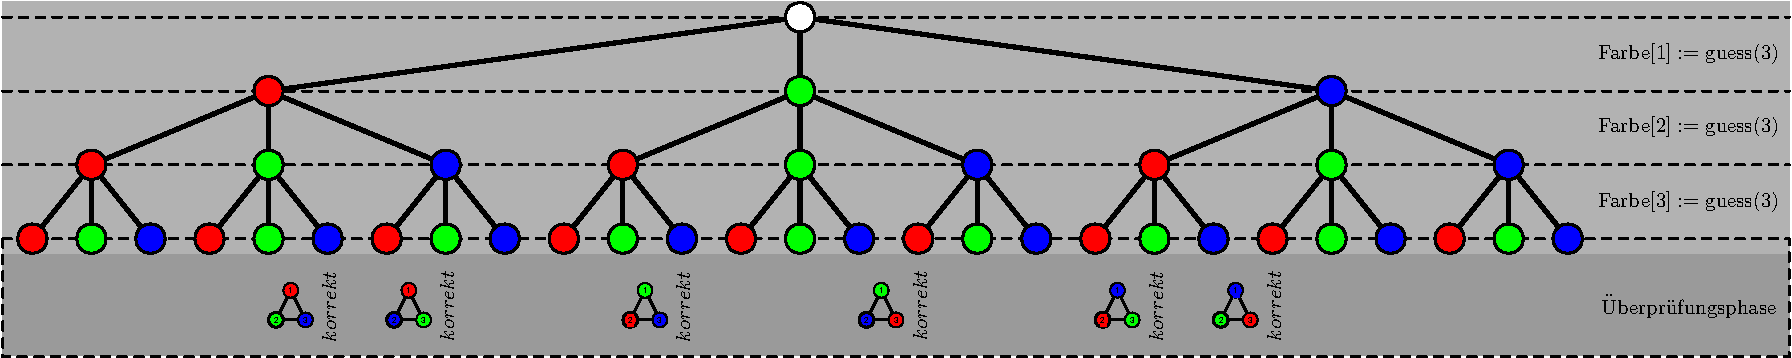
\includegraphics[scale=0.45]{NDetTree}}
\caption{Ein Berechnungsbaum für das $3\mathrm{COL}$-Problem}
\label{Tree3COL}
\end{figure}
%
An den Kanten des Baumes findet sich das Resultat der Rateanweisung
der darüberliegenden Verzweigung. Jeder Pfad in diesem sogenannten
\dindex{Berechnungsbaum} entspricht daher einer Folge von
Farbzuordnungen an die Knoten, d.h.~einer potenziellen Färbung. Der
Graph ist $3$-färbbar, falls sich auf mindestens einem Pfad eine
korrekte Färbung ergibt, falls also auf mindestens einem Pfad die
Überprüfungsphase\index{Uberprüfungsphase=Überprüfungsphase} 
erfolgreich ist; der Beispielgraph besitzt sechs korrekte $3$-Färbungen, 
ist also eine positive Instanz des $3\mathrm{COL}$-Problems.

Eine weitere, vielleicht intuitivere Vorstellung für die Arbeitsweise
dieser $\NP$-Ma\-schi\-ne ist die, dass bei jedem Ratevorgang $3$
verschiedene unabhängige Prozesse gestartet werden, die aber nicht
miteinander kommunizieren dürfen. In diesem Sinne hat man es hier mit
einem eingeschränkten Parallelrechner zu tun: Beliebige Aufspaltung
(fork) ist erlaubt, aber keine Kommunikation zwischen den Prozessen
ist möglich. Würde man Kommunikation zulassen, hätte man erneut den
allgemeinen Parallelrechner mit exponentiell vielen Prozessoren von
oben, der sich ja als zu mächtig für $\NP$ herausgestellt hat.

Es hat sich also gezeigt, dass eine Art "`Rateanweisung"' benötigt
wird. In der Programmiersprache für $\NP$ verwendet man dazu das neue
Schlüsselwort $\mathbf{guess}(m)$, wobei $m$ die Anzahl von
Möglichkeiten ist, aus denen eine geraten wird, und legt fest, dass
auch die Anweisung $\mathbf{guess}(m)$ nur einen Takt Zeit für ihre
Abarbeitung benötigt.  Berechnungen, die, wie soeben beschrieben,
verschiedene Möglichkeiten raten können, heißen
\dindex{nichtdeterministisch}. Es sei wiederholt, dass \emph{festgelegt}
(definiert) wird, dass ein nichtdeterministischer Algorithmus bei
einer Eingabe den Wert $1$ berechnet, falls \emph{eine
Möglichkeit} geraten werden kann, sodass der Algorithmus auf die
Anweisung "`\textbf{return} $1$"' stößt. Die Klasse $\NP$
umfasst nun genau die Probleme, die von nichtdeterministischen
Algorithmen mit polynomieller Laufzeit gelöst werden können.
"`$\NP$"' steht dabei für
"`\textbf{n}ichtdeterministi\-sche \textbf{P}olynomialzeit"', nicht
etwa, wie mitunter zu lesen, für "`Nicht-Polynomialzeit"'.  (Eine
formale Präsentation der Äquivalenz zwischen effizienter
Überprüfbarkeit und Polynomialzeit in der $\NP$-Pro\-gram\-miersprache
findet sich z.B.~in \cite[Kapitel 2.3]{GaJo79}.)

Mit Hilfe eines nichtdeterministischen Algorithmus kann das
$3\mathrm{COL}$-Problem in Polynomialzeit gelöst werden (siehe
Algorithmus \ref{3COLAlgo}). Die zweite Phase von
Algorithmus \ref{3COLAlgo}, die
\emph{Überprüfungsphase}\index{Uberprüfungsphase=Überprüfungsphase}, 
entspricht dabei genau dem oben angegebenen Algorithmus zum
effizienten Überprüfen von möglichen Lösungen des
$3\mathrm{COL}$-Problems (vgl.~Algorithmus \ref{TestCOL}).

\RestyleAlgo{ruled}
\begin{algorithm}
\caption{Ein nichtdeterministischer Algorithmus für $3\mathrm{COL}$}
\label{3COLAlgo}
\KwData{Graph $G = (\{v_1, \dots v_n\}, E)$}
\KwResult{$1$ wenn eine Färbung existiert, $0$ sonst}
\BlankLine
\Begin{
    \tcc*[f]{Ratephase}

    \For{$(i = 1$ $\mathrm{to}$ $n)$}{
        $\mathrm{Farbe}[i] = \mathrm{guess}(3)$\;
    }
    \tcc*[f]{Überprüfungsphase}

    \For{$(i = 1$ $\mathrm{to}$ $n)$}{
      \For{$(j = 1$ $\mathrm{to}$ $n)$}{
        \If{$(((v_i,v_j) \in E)$ $\mathrm{und}$ $(v_i \text{ und }
            v_j \text{ sind gleich gefärbt}))$}{
          \Return $0$\;
        }
      }
    }
  \Return $1$\;
  }
\end{algorithm}

Dieser nichtdeterministische Algorithmus läuft in Polynomialzeit, denn
man benötigt für einen Graphen mit $n$ Knoten mindestens $n$ Bits, um
ihn zu speichern (kodieren), und der Algorithmus braucht im
schlechtesten Fall $O(n)$ (Ratephase) und $O(n^2)$
(Überprüfungsphase), also insgesamt $O(n^2)$ Takte Zeit.  Damit ist
gezeigt, dass $3\mathrm{COL}$ in der Klasse $\NP$ enthalten ist, denn
es wurde ein nichtdeterministischer Polynomialzeitalgorithmus
gefunden, der $3\mathrm{COL}$ löst. Ebenso einfach könnte man nun
einen nichtdeterministischen Polynomialzeitalgorithmus entwickeln, der
das Problem \textsf{HAMILTON} löst: Der Algorithmus wird in einer
ersten Phase eine Knotenfolge raten und dann in einer zweiten Phase
überprüfen, dass die Bedingungen, die an einen Hamiltonschen Kreis
gestellt werden, bei der geratenen Folge erfüllt sind. Dies zeigt,
dass auch \textsf{HAMILTON} in der Klasse $\NP$ liegt.

Dass eine nichtdeterministische Maschine nicht gebaut werden kann,
spielt hier keine Rolle. Nichtdeterministische Berechnungen sollen
hier lediglich als Gedankenmodell für unsere Untersuchungen
herangezogen werden, um Aussagen über die (Nicht-) Existenz von
effizienten Algorithmen machen zu können.

\subsection{Schwierigste Probleme in $\mathbf{NP}$: der Begriff der 
$\mathbf{NP}$-Vollständigkeit}

Es ist nun klar, was es bedeutet, dass ein Problem in $\NP$ liegt. Es
liegt aber auch auf der Hand, dass alle Probleme aus $\P$ auch in
$\NP$ liegen, da bei der Einführung von $\NP$ ja nicht verlangt wurde,
dass die $\mathbf{guess}$-Anweisung verwendet werden muss. Damit ist
jeder deterministische Algorithmus automatisch auch ein
(eingeschränkter) nichtdeterministischer Algorithmus. Nun ist aber
auch schon bekannt, dass es Probleme in $\NP$ gibt, z.B.~$3\mathrm{COL}$ und
weitere Probleme, von denen nicht bekannt ist, ob sie in $\P$
liegen. Das führt zu der Vermutung, dass $\P\neq\NP$.

Es gibt also in $\NP$ anscheinend unterschiedlich schwierige Probleme:
einerseits die $\P$-Probleme (also die leichten Probleme), und
andererseits die Probleme, von denen man nicht weiß, ob sie in $\P$
liegen (die schweren Probleme).  Es liegt also nahe, eine allgemeine
Möglichkeit zu suchen, Probleme in $\NP$ bezüglich ihrer Schwierigkeit
zu vergleichen. Ziel ist, wie oben erläutert, eine Art von unterer
Schranke für Probleme wie $3\mathrm{COL}$: Es soll gezeigt werden,
dass $3\mathrm{COL}$ mindestens so schwierig ist, wie jedes andere
Problem in $\NP$, also in gewissem Sinne ein \emph{schwierigstes
Problem in $\NP$} ist.

Für diesen Vergleich der Schwierigkeit ist die erste Idee natürlich,
einfach die Laufzeit von (bekannten) Algorithmen für das Problem
heranzuziehen. Dies ist jedoch nicht erfolgversprechend, denn was soll
eine "`größte"' Laufzeit sein, die Programme für "`schwierigste"'
Probleme in $\NP$ ja haben müssten?  Außerdem hängt die Laufzeit eines
Algorithmus vom verwendeten Berechnungsmodell ab. So kennen
Turingmaschinen keine Arrays im Gegensatz zu der hier verwendeten
C-Variante. Also würde jeder Algorithmus, der Arrays verwendet,
auf einer Turingmaschine mühsam simuliert werden müssen und damit
langsamer abgearbeitet werden, als bei einer Hochsprache, die Arrays
enthält. Obwohl sich die Komplexität eines Problems nicht ändert,
würde man sie verschieden messen, je nachdem welches Berechnungsmodell
verwendet würde. Ein weiterer Nachteil dieses Definitionsversuchs wäre
es, dass die Komplexität (Schwierigkeit) eines Problems mit bekannten
Algorithmen gemessen würde. Das würde aber bedeuten, dass jeder neue
und schnellere Algorithmus Einfluss auf die Komplexität hätte, was
offensichtlich so keinen Sinn macht.  Aus diesen und anderen Gründen
führt die erste Idee nicht zum Ziel.

Eine zweite, erfolgversprechendere Idee ist die folgende: Ein Problem
$A$ ist nicht (wesentlich) schwieriger als ein Problem $B$, wenn man
$A$ mit der Hilfe von $B$ (als Unterprogramm) effizient lösen
kann. Ein einfaches Beispiel ist die Multiplikation von $n$ Zahlen.
Angenommen, man hat schon ein Programm, dass zwei Zahlen multiplizieren
kann; dann ist es nicht wesentlich schwieriger, auch $n$ Zahlen zu
multiplizieren, wenn die Routine für die Multiplikation von zwei Zahlen
verwendet wird. Dieser Ansatz ist unter dem Namen \emph{relative
  Berechenbarkeit} bekannt, der genau den oben beschriebenen
Sachverhalt widerspiegelt: Multiplikation von $n$ Zahlen (so genannte
\emph{iterierte Multiplikation}) ist relativ zur Multiplikation zweier
Zahlen (leicht) berechenbar.

Da das Prinzip der relativen Berechenbarkeit so allgemein gehalten
ist, gibt es innerhalb der theoretischen Informatik sehr viele
verschiedene Ausprägungen dieses Konzepts. Für die
$\P$-$\NP$-Problematik ist folgende Version der relativen
Berechenbarkeit, d.h.~die folgende Art von erlaubten
"`Unterprogrammaufrufen"', geeignet:\\
%
Seien zwei Probleme $A$ und $B$ gegeben. Das Problem $A$ ist nicht
schwerer als $B$, falls es eine effizient zu berechnende
Transformation $T$ gibt, die Folgendes leistet: Wenn $x$ eine
Eingabeinstanz von Problem $A$ ist, dann ist $T(x)$ eine
Eingabeinstanz für $B$. Weiterhin gilt: $x$ ist \emph{genau dann} eine
positive Instanz von $A$ (d.h.~ein Entscheidungsalgorithmus für $A$
muss den Wert $1$ für Eingabe $x$ liefern), wenn $T(x)$ eine positive
Instanz von Problem $B$ ist. Erneut soll "`effizient berechenbar"'
hier bedeuten: in Polynomialzeit berechenbar. Es muss also einen
Polynomialzeitalgorithmus geben, der die Transformation $T$ ausführt.
Das Entscheidungsproblem $A$ ist damit effizient transformierbar in
das Problem $B$. Man sagt auch: $A$ ist reduzierbar auf $B$; oder
intuitiver: $A$ ist nicht schwieriger als $B$, oder $B$ ist mindestens
so schwierig wie $A$. Formal schreibt man dann $A\leq B$.

Um für dieses Konzept ein wenig mehr Intuition zu gewinnen, sei
erwähnt, dass man sich eine solche Transformation auch wie folgt
vorstellen kann: $A$ lässt sich auf $B$ reduzieren, wenn ein
Algorithmus für $A$ angegeben werden kann, der ein Unterprogramm $U_B$
für $B$ genau so verwendet wie in Algorithmus \ref{RedAlgo} gezeigt.

Dabei ist zu beachten, dass das Unterprogramm für $B$ nur genau einmal
und zwar am Ende aufgerufen werden darf.  Das Ergebnis des Algorithmus
für $A$ ist genau das Ergebnis, das dieser Unterprogrammaufruf
liefert.  Es gibt zwar, wie oben erwähnt, auch allgemeinere
Ausprägungen der relativen Berechenbarkeit, die diese Einschränkung
nicht haben, diese sind aber für die folgenden Untersuchungen nicht
relevant.

Nachdem nun ein Vergleichsbegriff für die Schwierigkeit von Problemen
aus $\NP$ gefunden wurde, kann auch definiert werden, was unter einem
"`schwierigsten"' Problem in $\NP$ zu verstehen ist. Ein Problem $C$
ist ein schwierigstes Problem in $\NP$, wenn alle anderen Probleme in
$\NP$ höchstens so schwer wie $C$ sind. Formaler ausgedrückt sind dazu
zwei Eigenschaften von $C$ nachzuweisen:

\begin{enumerate}[{\sffamily(1)}]
\item $C$ ist ein Problem aus $\NP$.
\item $C$ ist mindestens so schwierig wie jedes andere $\NP$-Problem
$A$; d.h.: für alle Probleme $A$ aus $\NP$ gilt: $A \le C$.
\end{enumerate}

\RestyleAlgo{ruled}
\begin{algorithm}
\caption{Algorithmische Darstellung der Benutzung einer Reduktionsfunktion}
\label{RedAlgo}
%
\KwData{Instanz $x$ für das Problem $A$}
\KwResult{$1$ wenn $x \in A$ und $0$ sonst}
\BlankLine
\Begin{
\tcc*[f]{$T$ ist die Reduktionsfunktion (polynomialzeitberechenbar)}

berechne $y = T(x)$\;
\tcc*[f]{$y$ ist Instanz des Problems $B$}

$z = U_B(y)$\;

\tcc*[f]{$z$ ist $1$ genau dann, wenn $x \in A$ gilt}

\Return $z$\;
}
\end{algorithm}

Solche schwierigsten Probleme in $\NP$ sind unter der Bezeichnung
\emph{$\NP$-vollständige Probleme}\index{vollständig}
bekannt. Nun sieht die Aufgabe, von einem Problem zu zeigen, dass es
$\NP$-vollständig ist, ziemlich hoffnungslos aus. Immerhin ist zu
zeigen, dass für alle Probleme aus $\NP$ -- und damit unendlich viele
-- gilt, dass sie höchstens so schwer sind wie das zu untersuchende
Problem, und damit scheint man der Schwierigkeit beim Nachweis unterer
Schranken nicht entgangen zu sein. Dennoch konnten der russische
Mathematiker Leonid Levin und der amerikanische Mathematiker Stephen
Cook Anfang der siebziger Jahre des letzten Jahrhunderts unabhängig
voneinander die Existenz von solchen $\NP$-vollständigen Problemen
zeigen. Hat man nun erst einmal \emph{ein} solches Problem
identifiziert, ist die Aufgabe, \emph{weitere} $\NP$-vollständige
Probleme zu finden, wesentlich leichter. Dies ist sehr leicht
einzusehen: Ein $\NP$-Problem $C$ ist ein schwierigstes Problem in
$\NP$, wenn es ein anderes schwierigstes Problem $B$ gibt, sodass $C$
nicht leichter als $B$ ist.  Das führt zu folgendem "`Kochrezept"':
\medskip

\noindent{\sffamily\bfseries Nachweis der $\NP$-Vollständigkeit 
eines Problems $C$:}
\begin{enumerate}[i)]
\item Zeige, dass $C$ in $\NP$ enthalten ist, indem dafür ein
geeigneter nichtdeterministischer Polynomialzeitalgorithmus
konstruiert wird.
\item Suche ein geeignetes "`ähnliches"' schwierigstes Problem $B$ in
$\NP$ und zeige, dass $C$ nicht leichter als $B$ ist. Formal: Finde ein
$\NP$-vollständiges Problem $B$ und zeige $B \le C$ mit Hilfe einer
geeigneten Transformation $T$.
\end{enumerate}

Den zweiten Schritt kann man oft relativ leicht mit Hilfe von
bekannten Sammlungen $\NP$-vollständiger Problemen erledigen. Das Buch
von Garey und Johnson \cite{GaJo79} ist eine solche Sammlung (siehe
auch die Abbildungen \ref{NPVollProbs1} und \ref{NPVollProbs2}), die
mehr als $300$ $\NP$-vollständige Probleme enthält. Dazu wählt man ein
möglichst ähnliches Problem aus und versucht dann eine geeignete
Reduktionsfunktion für das zu untersuchende Problem zu finden.

\goodbreak
\subsubsection{Traveling Salesperson ist $\mathbf{NP}$-vollständig}
Wie kann man zeigen, dass Traveling Salesperson $\NP$-vollständig ist?
Dazu wird zuerst die genaue Definition dieses Problems benötigt:

\dprob{TRAVELING SALESPERSON (TSP)}%
{Eine Menge von Städten $C = \{c_1, \dots ,c_n \}$ und eine $n \times
  n$ Entfernungsmatrix $D$, wobei das Element $D[i,j]$ der Matrix $D$
  die Entfernung zwischen Stadt $c_i$ und $c_j$ angibt. Weiterhin eine
  Obergrenze $k \ge 0$ für die maximal erlaubte Länge der Tour}%
{Gibt es eine Rundreise, die einerseits alle Städte besucht, aber
  andererseits eine Gesamtlänge von höchstens $k$ hat?}

Nun zum ersten Schritt des Nachweises der $\NP$-Vollständigkeit von
\textsf{TSP}: Offensichtlich gehört auch das Traveling Salesperson Problem zur
Klasse $\NP$, denn man kann nichtdeterministisch eine Folge von $n$
Städten raten (eine potenzielle Rundreise) und dann leicht überprüfen,
ob diese potenzielle Tour durch alle Städte verläuft und ob die
zurückzulegende Entfernung maximal $k$ beträgt. Ein entsprechender
nichtdeterministischer Polynomialzeitalgorithmus ist leicht zu
erstellen. Damit ist der erste Schritt zum Nachweis der
$\NP$-Vollständigkeit von \textsf{TSP} getan und Punkt (1) des
"`Kochrezepts"' abgehandelt.

Als nächstes (Punkt (2)) soll von einem anderen $\NP$-vollständigen
Problem gezeigt werden, dass es effizient in \textsf{TSP}
transformiert werden kann. Geeignet dazu ist das im Text betrachtete
Hamitonkreis-Problem, das bekanntermaßen $\NP$-vollständig ist. Es
ist also zu zeigen: \textsf{HAMILTON} $\le$ \textsf{TSP}.

Folgende Idee führt zum Ziel: Gegeben ist eine Instanz $G=(V,E)$ von
\textsf{HAMILTON}. Transformiere $G$ in folgende Instanz von \textsf{TSP}: Als
Städtemenge $C$ wählen wir die Knoten $V$ des Graphen $G$. Die
Entfernungen zwischen den Städten sind definiert wie folgt:
$D[i,j]=1$, falls es in $E$ eine Kante von Knoten $i$ zu Knoten $j$
gibt, ansonsten setzt man $D[i,j]$ auf einen sehr großen Wert, also
z.B. $n+1$, wenn $n$ die Anzahl der Knoten von $G$ ist. Dann gilt
klarerweise: Wenn $G$ einen Hamiltonschen Kreis besitzt, dann ist der
gleiche Kreis eine Rundreise in $C$ mit Gesamtlänge $n$.  Wenn $G$
keinen Hamiltonschen Kreis besitzt, dann kann es keine Rundreise durch
die Städte $C$ mit Länge höchstens $n$ geben, denn jede Rundreise muss
mindestens eine Strecke von einer Stadt $i$ nach einer Stadt $j$
zurücklegen, die keiner Kante in $G$ entspricht (denn ansonsten hätte
$G$ ja einen Hamiltonschen Kreis). Diese einzelne Strecke von $i$ nach
$j$ hat dann aber schon Länge $n+1$ und damit ist eine Gesamtlänge von
$n$ oder weniger nicht mehr erreichbar. Die Abbildung \ref{TSPRedExample} 
zeigt zwei Beispiele für die Wirkungsweise der Transformation, die
durch Algorithmus \ref{TSPRed} in Polynomialzeit berechnet wird.

\begin{figure}
\begin{center}
\fbox{
\begin{minipage}{0.93\textwidth}
\begin{minipage}{0.46\textwidth}
Aus dem Graphen $G$ links berechnet die Transformation die rechte
Eingabe für das \textsf{TSP}. Die dick gezeichneten Verbindungen deuten
eine Entfernung von $1$ an, wogegen dünne Linien eine Entfernung
von $6$ symbolisieren. Weil $G$ den Hamiltonkreis $1,2,3,4,5,1$ hat,
gibt es rechts eine Rundreise $1,2,3,4,5,1$ mit Gesamtlänge $5$.
\end{minipage}
\begin{minipage}{0.46\textwidth}
\centerline{\hspace*{3em}\includegraphics[scale=0.40]{CG1.eps}}
\end{minipage}

\bigskip

\begin{minipage}{0.46\textwidth}
Im Gegensatz dazu berechnet die Transformation hier aus dem Graphen
$G'$ auf der linken eine Eingabe für das \textsf{TSP} auf der rechten
Seite, die, wie man sich leicht überzeugt, keine Rundreise mit einer
maximalen Gesamtlänge von $5$ hat. Dies liegt daran, dass der
ursprüngliche Graph $G'$ keinen Hamiltonschen Kreis hatte.
\end{minipage}
\begin{minipage}{0.46\textwidth}
\centerline{\hspace*{3em}\includegraphics[scale=0.40]{CG2.eps}}
\end{minipage}
\end{minipage}
}
\end{center}
\caption[Beispiele für die Wirkungsweise von Algorithmus \ref*{TSPRed}]{Beispiele für die Wirkungsweise von Algorithmus \ref{TSPRed}}
\label{TSPRedExample}
\end{figure}

\RestyleAlgo{ruled}
\begin{algorithm}
\caption{Ein Algorithmus für die Reduktion von \textsf{HAMILTON} auf \textsf{TSP}}
\label{TSPRed}
\KwData{Graph $G=(V, E)$, wobei $V = \set{\range{1}{n}}$}
\KwResult{Eine Instanz $(C, D, k)$ für \textsf{TSP}}
\BlankLine
\Begin{
    \tcc*[f]{Die Knoten entsprechen den Städten}

    $C = V$\;       

    \tcc*[f]{Überprüfe alle potentiell existierenden Kanten}
    
    \For{$(i = 1$ $\mathrm{to}$ $n)$}{
      \For{$(j = 1$ $\mathrm{to}$ $n)$}{
        \uIf{$((v_i,v_j) \in E)$}{%
            \tcc*[f]{Kanten entsprechen kleinen Entfernungen}

            $D[i][j] = 1$\;       
         }
         \Else{%
            \tcc*[f]{nicht existierende Kante, dann sehr große Entfernung}

            $D[i][j] = n + 1$\;       
         }
        }
      }
      \tcc*[f]{Gesamtlänge $k$ der Rundreise ist Anzahl der Städte $n$}

      $k = n$\;
      \tcc*[f]{Gebe die berechnete \textsf{TSP}-Instanz zurück}

      \Return $(C,D,k)$\;
}
\end{algorithm}

\subsection{Die Auswirkungen der $\mathbf{NP}$-Vollständigkeit}
Welche Bedeutung haben nun die $\NP$-vollstän\-digen Probleme für die
Klasse $\NP$? Könnte jemand einen deterministischen
Polynomialzeitalgorithmus $\mathcal{A}_C$ für ein
$\NP$-voll\-stän\-diges Problem $C$ angeben, dann hätte man für jedes
$\NP$-Problem einen Polynomialzeitalgorithmus gefunden
(d.h.~$\P=\NP$). Diese überraschende Tatsache lässt sich leicht
einsehen, denn für jedes Problem $A$ aus $\NP$ gibt es eine
Transformation $T$ mit der Eigenschaft, dass $x$ genau dann eine
positive Eingabeinstanz von $A$ ist, wenn $T(x)$ eine positive Instanz
von $C$ ist. Damit löst Algorithmus \ref{PolyAlgoNP} das Problem $A$
in Polynomialzeit. Es gilt also: Ist irgendein $\NP$-vollstän\-diges
Problem effizient lösbar, dann ist $\P=\NP$.

\RestyleAlgo{ruled}
\begin{algorithm}
\caption{Ein fiktiver Algorithmus für Problem $A$}
\label{PolyAlgoNP}
\KwData{Instanz $x$ für das Problem $A$}
\KwResult{\texttt{true}, wenn $x \in A$, \texttt{false} sonst}
\BlankLine
\Begin{
   \tcc*[f]{$T$ ist die postulierte Reduktionsfunktion}

   $y = T(x)$\;
   $z =\mathcal{A}_C(y)$\;
   \BlankLine
   \Return $z$\;
}
\end{algorithm}

Sei nun angenommen, dass jemand $\P \not= \NP$ gezeigt hat. In diesem
Fall ist aber auch klar, dass dann für kein $\NP$-vollständiges
Problem ein Polynomialzeitalgorithmus existieren kann, denn sonst
würde sich ja der Widerspruch $\P = \NP$ ergeben.  Ist das Problem $C$
also $\NP$-vollständig, so gilt: $C$ hat genau dann einen effizienten
Algorithmus, wenn $\P=\NP$, also wenn jedes Problem in $\NP$ einen
effizienten Algorithmus besitzt. Diese Eigenschaft macht die
$\NP$-vollständigen Probleme für die Theoretiker so interessant, denn
eine Klasse von unendlich vielen Problemen kann untersucht werden,
indem man nur ein einziges Problem betrachtet. Man kann sich das auch
wie folgt vorstellen: Alle relevanten Eigenschaften aller Probleme aus
$\NP$ wurden in ein einziges Problem "`destilliert"'. Die
$\NP$-vollständigen Probleme sind also in diesem Sinn
\emph{prototypische} $\NP$-Probleme.

Trotz intensiver Bemühungen in den letzten 30 Jahren konnte bisher
niemand einen Polynomialzeitalgorithmus für ein $\NP$-vollständiges
Problem finden. Dies ist ein Grund dafür, dass man heute
$\P \not= \NP$ annimmt. Leider konnte auch dies bisher nicht gezeigt
werden, aber in der theoretischen Informatik gibt es starke Indizien
für die Richtigkeit dieser Annahme, sodass heute die große Mehrheit
der Forscher von $\P
\not= \NP$ ausgeht.

Für die Praxis bedeutet dies Folgendes: Hat man von einem in der
Realität auftretenden Problem gezeigt, dass es $\NP$-vollständig ist,
dann kann man getrost aufhören, einen effizienten Algorithmus zu
suchen. Wie wir ja gesehen haben, kann ein solcher nämlich (zumindest
unter der gut begründbaren Annahme $\P\neq\NP$) nicht existieren.

Nun ist auch eine Antwort für das $3\mathrm{COL}$-Problem gefunden. Es wurde
gezeigt \cite{GaJo79}, dass $k\mathrm{COL}$ für $k \ge 3$ $\NP$-vollständig
ist. Der fiktive Mobilfunkplaner hat also Pech gehabt: Es ist
unwahrscheinlich, dass er jemals ein korrektes effizientes
Planungsverfahren finden wird.

Ein $\NP$-Vollständigkeitsnachweis eines Problems ist also ein starkes
Indiz für seine praktische Nicht-Handhabbarkeit. Auch die
$\NP$-Vollständigkeit eines Problems, das mit dem Spiel
\emph{Minesweeper} zu tun hat, bedeutet demnach
lediglich, dass dieses Problem höchstwahrscheinlich nicht effizient
lösbar sein wird. Ein solcher Vollständigkeitsbeweis hat nichts mit
einem Schritt in Richtung auf eine Lösung des
$\P\stackrel{?}{=}\NP$-Problems zu tun, wie irreführenderweise
gelegentlich zu lesen ist. Übrigens ist auch für eine Reihe weiterer
Spiele ihre $\NP$-Vollständigkeit bekannt. Dazu gehören {u.a.}
bestimmte Puzzle- und Kreuzwortspiele. Typische Brettspiele, wie Dame,
Schach oder GO, sind hingegen (verallgemeinert auf Spielbretter der
Größe $n\times n$) \textbf{PSPACE}-vollständig. Die Klasse
\textbf{PSPACE} ist eine noch deutlich mächtigere Klasse als
$\NP$. Damit sind also diese Spiele noch viel komplexer als
Minesweeper und andere $\NP$-vollständige Probleme.


\begin{figure}
\begin{center}
\footnotesize
Problemnummern in "`[\dots]"' beziehen sich auf die Sammlung von
Garey und Johnson \cite{GaJo79}.

\columnsep1em
\begin{multicols}{2}
\dprob{CLUSTER \textrm{[GT19]}}
{Netzwerk $G=(V,E)$, positive Integerzahl $K$}
{Gibt es eine Menge von mindestens $K$ Knoten, die paarweise miteinander
verbunden sind?}
%
\dprob{NETZ-AUFTEILUNG \textrm{[ND16]}}
{Netzwerk $G=(V,E)$, Kapazität für jede Kante in $E$, positive
Integerzahl $K$}
{Kann man das Netzwerk so in zwei Teile zerlegen, dass die Gesamtkapazität
aller Verbindungen zwischen den beiden Teilen mindestens $K$ beträgt?}
%
\dprob{NETZ-REDUNDANZ \textrm{[ND18]}}
{Netzwerk $G=(V,E)$, Kosten für Verbindungen zwischen je zwei Knoten aus 
$V$, Budget $B$}
{Kann $G$ so um Verbindungen erweitert werden, dass zwischen je zwei Knoten
mindestens zwei Pfade existieren und die Gesamtkosten für die Erweiterung
höchstens $B$ betragen?}
%
\dprob{OBJEKTE SPEICHERN \textrm{[SR1]}}
{Eine Menge $U$ von Objekten mit Speicherbedarf $s(u)$ für jedes $u \in U$;
Kachelgröße $S$, positive Integerzahl $K$}
{Können die Objekte in $U$ auf $K$ Kacheln verteilt werden?}
%
\dprob{DATENKOMPRESSION \textrm{[SR8]}}
{Endliche Menge $R$ von Strings über festgelegtem Alphabet, positive
Integerzahl $K$}
{Gibt es einen String $S$ der Länge höchstens $K$, sodass jeder String aus $R$
als Teilfolge von $S$ vorkommt?}
%
\dprob{$K$-SCHLÜSSEL \textrm{[SR26]}}
{Relationales Datenbankschema, gegeben durch Attributmenge $A$ und
funktionale Abhängigkeiten auf $A$, positive Integerzahl $K$}
{Gibt es einen Schlüssel mit höchstens $K$ Attributen?}
%
\goodbreak
%
\dprob{BCNF \textrm{[SR29]}}
{Relationales Datenbankschema, gegeben durch Attributmenge $A$ und
funktionale Abhängigkeiten auf $A$, Teilmenge $A' \subseteq A$}
{Verletzt die Menge $A'$ die Boyce-Codd-Normalform?}
%
\dprob{MP-SCHEDULE \textrm{[SS8]}}
{Menge $T$ von Tasks, Länge für jede Task, Anzahl $m$ von Prozessoren, 
positive Integerzahl $D$ ("`Deadline"')}
{Gibt es ein $m$-Prozessor-Schedule für $T$ mit Ausführungszeit höchstens
$D$?}
%
\dprob{PREEMPT-SCHEDULE \textrm{[SS12]}}
{Menge $T$ von Tasks, Länge für jede Task, Präzedenzrelation auf den
Tasks, Anzahl $m$ von Prozessoren, positive Integerzahl $D$
("`Deadline"')}
{Gibt es ein $m$-Prozessor-Schedule für $T$, das die
Präzedenzrelationen berücksichtigt und Ausführungszeit höchstens $D$
hat?}
%
\dprob{DEADLOCK \textrm{[SS22]}}
{Menge von Prozessen, Menge von Ressourcen, aktuelle Zustände der 
Prozesse und aktuell allokierte Ressourcen}
{Gibt es einen Kontrollfluss, der zum Deadlock führt?}
%
\dprob{$K$-REGISTER \textrm{[PO3]}}
{Menge $V$ von Variablen, die in einer Schleife benutzt werden, für jede
Variable einen Gültigkeitsbereich, positive Integerzahl $K$}
{Können die Schleifenvariablen mit höch\-stens $K$ Registern gespeichert werden?}
%
\dprob{REKURSION \textrm{[PO20]}}
{Menge $A$ von Prozedur-Identifiern, Pascal-Programm\-fragment mit
Deklarationen und Aufrufen der Prozeduren aus $A$}
{Ist eine der Prozeduren aus $A$ formal rekursiv?}
\end{multicols}
\end{center}
\caption{Eine kleine Sammlung $\NP$-vollständiger Probleme (Teil 1)}
\label{NPVollProbs1}
\end{figure}

\begin{figure}
\begin{center}
\footnotesize
Problemnummern in "`[\dots]"' beziehen sich auf die Sammlung von
Garey und Johnson \cite{GaJo79}.

\columnsep1em
\begin{multicols}{2}
\dprob{LR($K$)-GRAMMATIK \textrm{[AL15]}}
{Kontextfreie Grammatik $G$, positive Integerzahl $K$ (unär)}
{Ist die Grammatik $G$ nicht LR($K$)?}
%
\dprob{ZWANGSBEDINGUNG \textrm{[LO5]}}
{Menge von Booleschen Constraints, positive Integerzahl $K$}
{Können mindestens $K$ der Constraints gleichzeitig erfüllt werden?}
%
\dprob{INTEGER PROGRAM \textrm{[MP1]}}
{Lineares Programm}
{Hat das Programm eine Lösung, die nur ganzzahlige Werte enthält?}
%
\dprob{KREUZWORTRÄTSEL \textrm{[GP15]}}%
{Menge $W$ von Wörtern, Gitter mit schwarzen und weißen Feldern}
{Können die weißen Felder des Gitters mit Wörtern aus $W$ gefüllt werden?}%
\end{multicols}
\caption{Eine kleine Sammlung $\NP$-vollständiger Probleme (Teil 2)}
\label{NPVollProbs2}
\end{center}
\end{figure}

\subsection{Der Umgang mit $\mathbf{NP}$-vollständigen Problemen in der Praxis}

Viele in der Praxis bedeutsame Probleme sind $\NP$-vollständig
(vgl.~die Abbildungen \ref{NPVollProbs1} und \ref{NPVollProbs2}). Ein
Anwendungsentwickler wird es aber sicher schwer haben, seinem
Management mitteilen zu müssen, dass ein aktuelles Projekt nicht
durchgeführt werden kann, weil keine geeigneten Algorithmen zur
Verfügung stehen (Wahrscheinlich würden in diesem Fall einfach
"`geeignetere"' Entwickler eingestellt werden!). Es stellt sich daher
also die Frage, wie man mit solchen $\NP$-vollständigen Problemen in
der Praxis umgeht. Zu dieser Fragestellung hat die theoretische
Informatik ein ausgefeiltes Instrumentarium entwickelt.

Eine erste Idee wäre es, sich mit Algorithmen zufrieden zu geben, die
mit Zufallszahlen arbeiten und die nur mit sehr großer
Wahrscheinlichkeit die richtige Lösung berechnen, aber sich auch mit
kleiner (vernachlässigbarer) Wahrscheinlichkeit irren dürfen. Solche
Algorithmen sind als \emph{probabilistische} oder \emph{randomisierte
Algorithmen}\index{Algorithmus!probabilistisch}\index{Algorithmus!randomisiert}
bekannt \cite{mora95} und werden beispielsweise in der Kryptographie
mit sehr großem Erfolg angewendet.  Das prominenteste Beispiel hierfür
sind Algorithmen, die testen, ob eine gegebene Zahl eine Primzahl ist
und sich dabei fast nie irren. Primzahlen spielen bekanntermaßen im
RSA-Verfahren und damit bei PGP und ähnlichen Verschlüsselungen eine
zentrale Rolle.  Es konnte aber gezeigt werden, dass probabilistische
Algorithmen uns bei den $\NP$-vollständigen Problemen wohl nicht
weiterhelfen. So weiß man heute, dass die Klasse der Probleme, die
sich mit probabilistischen Algorithmen effizient lösen lässt,
höchstwahrscheinlich nicht die Klasse $\NP$ umfasst. Deshalb liegen
(höchstwahrscheinlich) insbesondere alle $\NP$-vollständigen Probleme
außerhalb der Möglichkeiten von effizienten probabilistischen
Algorithmen.

Nun könnte man auch versuchen, "`exotischere"' Computer zu bauen.  In
der letzten Zeit sind zwei potenzielle Auswege bekannt geworden:
DNA-Computer und Quantencomputer.

Es konnte gezeigt werden, dass DNA-Computer (siehe \cite{pau98}) jedes
$\NP$-vollständige Problem in Polynomialzeit lösen können. Für diese
Berechnungsstärke hat man aber einen Preis zu zahlen: Die Anzahl und
damit die Masse der DNA-Moleküle, die für die Berechnung benötigt
werden, wächst exponentiell in der Eingabelänge. Das bedeutet, dass
schon bei recht kleinen Eingaben mehr Masse für eine Berechnung
gebraucht würde, als im ganzen Universum vorhanden ist. Bisher ist
kein Verfahren bekannt, wie dieses Masseproblem gelöst werden kann,
und es sieht auch nicht so aus, als ob es gelöst werden kann, wenn $\P
\not= \NP$ gilt. Dieses Problem erinnert an das oben im Kontext von
Parallelrechnern schon erwähnte Phänomen: Mit exponentiell vielen
Prozessoren lassen sich $\NP$-vollständige Probleme lösen, aber solche
Parallelrechner haben natürlich explodierende Hardware-Kosten.
 
Der anderer Ausweg könnten Quantencomputer sein
(siehe \cite{Ho08,gru99}). Hier scheint die Situation zunächst günstiger zu
sein: Die Fortschritte bei der Quanten\-computer-Forschung verlaufen
immens schnell, und es besteht die berechtigte Hoffnung, dass
Quantencomputer mittelfristig verfügbar sein werden. Aber auch hier
sagen theoretische Ergebnisse voraus, dass Quantencomputer
(höchstwahrscheinlich) keine $\NP$-vollständigen Probleme lösen
können. Trotzdem sind Quantencomputer interessant, denn es ist
bekannt, dass wichtige Probleme existieren, für die kein
Polynomialzeitalgorithmus bekannt ist und die wahrscheinlich nicht
$\NP$-vollständig sind, die aber auf Quantencomputern effizient gelöst
werden können. Das prominenteste Beispiel hierfür ist die Aufgabe,
eine ganze Zahl in ihre Primfaktoren zu zerlegen.

\goodbreak
Die bisher angesprochenen Ideen lassen also die Frage, wie man mit
$\NP$-vollständigen Problemen umgeht, unbeantwortet. In der Praxis
gibt es im Moment zwei Hauptansatzpunkte: Die erste Möglichkeit ist
die, die Allgemeinheit des untersuchten Problems zu beschränken und
eine spezielle Version zu betrachten, die immer noch für die geplante
Anwendung ausreicht. Zum Beispiel sind Graphenprobleme oft einfacher,
wenn man zusätzlich fordert, dass die Knoten des Graphen in der
(Euklidischen) Ebene lokalisiert sind. Deshalb sollte die erste Idee
bei der Behandlung von $\NP$-vollständigen Problemen immer sein, zu
untersuchen, welche Einschränkungen man an das Problem machen kann,
ohne die praktische Aufgabenstellung zu verfälschen. Gerade diese
Einschränkungen können dann effiziente Algorithmen ermöglichen.

Die zweite Möglichkeit sind sogenannte
\dindex{Approximationsalgorithmen} (vgl.~\cite{ACGJNO99}). Die Idee
hier ist es, nicht die optimalen Lösungen zu suchen, sondern sich mit
einem kleinen garantierten Fehler zufrieden zu geben.  Dazu folgendes
Beispiel. Es ist bekannt, dass das \textsf{TSP} auch dann noch
$\NP$-vollständig ist, wenn man annimmt, dass die Städte in der
Euklidischen Ebene lokalisiert sind, d.h.~man kann die Städte in einer
fiktiven Landkarte einzeichnen, sodass die Entfernungen zwischen den
Städten proportional zu den Abständen auf der Landkarte sind.  Das ist
sicherlich in der Praxis keine einschränkende Abschwächung des
Problems und zeigt, dass die oben erwähnte Methode nicht immer zum
Erfolg führen muss: Hier bleibt auch das eingeschränkte Problem
$\NP$-vollständig. Aber für diese eingeschränkte \textsf{TSP}-Variante
ist ein Polynomialzeitalgorithmus bekannt, der immer eine Rundreise
berechnet, die höchstens um einen beliebig wählbaren Faktor schlechter
ist, als die optimale Lösung. Ein Chip-Hersteller, der bei der
Bestückung seiner Platinen die Wege der Roboterköpfe minimieren
möchte, kann also beschließen, sich mit einer Tour zufrieden zu geben,
die um 5 \% schlechter ist als die optimale. Für dieses Problem
existiert ein effizienter Algorithmus!  Dieser ist für die Praxis
völlig ausreichend.
